\documentclass{article}
\usepackage[a4paper, total={6in, 8in}]{geometry}
\usepackage{amsmath, amsfonts, yhmath}
\usepackage{amsthm}
\newtheorem*{dfntn*}{Definition}
\newtheorem*{rmrk*}{Remark}


\usepackage{enumitem}

\usepackage{graphicx}
\usepackage{./src/assets/custom}

% for table
\usepackage{tabulary,booktabs}

\usepackage{xcolor}
\definecolor{morange}{RGB}{255,127,14}
\definecolor{mblue}{RGB}{31,119,180}
\definecolor{mred}{RGB}{214,39,40}
\definecolor{mpurple}{RGB}{148,103,189}
\definecolor{mgreen}{RGB}{44,160,44}

\begin{document}

We thanks both reviewers for their detailed comments and suggestions. Here we point out how we addressed them (the comments of the reviewers are in black and our responses to them in {\color{mred} red}):

\section{Comments from Reviewer I}

\subsection*{Major Comments}
\begin{enumerate}
\item Regarding Section 1:
\begin{enumerate}[label=\arabic*.]
\item The variable t should not be called a ``time step'' since it represents continuous time.

    {\color{mred}We now call this ``time''}.

\item It would be clearer to use another notation than $\nabla$ for the Jacobian matrix (as it is, it can be confused with the gradient operator).

    {\color{mred}We changed $\nabla\varphi$ to $D\varphi$ etc.}

\item The remark below equation (4) should appear earlier.

    {\color{mred}We now write ``the flow $\varphi_f^t$, in addition to being invertible, is also volume-preserving'' and ``and therefore (by using that $\varphi^t$ is invertible)''}

\item Before equation (3), A is not defined (I guess it's any matrix-valued function).

    {\color{mred} We now write: ``For any matrix-valued function $A$ we further have''}

\item Equation (4) proves that the determinant is constant, not that it is equal to 1.

    {\color{mred} We added ``The determinant of $D\varphi^t$ is therefore constant and we further have $D\varphi^0 = 1$ because $\varphi^0$ is the identity. This proofs our assertion.''}

\end{enumerate}

\item Regarding Section 4:
\begin{enumerate}[label=\arabic*.]
\item I suggest using $\check{}$ instead of $\tilde{}$ for the inverse of $\hat{}$.

    {\color{mred} Done!}
\item I suggest adding $\check{Z} =$ after the $\mapsto$ sign in equation (14).

    {\color{mred} Done!}
\item Since the Cayley transform in such an integral part of your method, and since it is not completely classical, I suggest spending more time explaining it, and its properties, around equation (15).

    {\color{mred} We added the following: ``The Cayley transform maps skew-symmetric matrices to orthogonal matrices, so if $Y$ has the property that $Y^T = -Y,$ then we have $\sigma(Y)^T\sigma(Y) = \mathbb{I}.$ This can be easily shown:

    \begin{equation*}
    \begin{aligned}
    \frac{d}{dt}\Big|_{t=0}\sigma(tY)^T\sigma(tY) & = \frac{d}{dt}(\mathbb{I}_{T} - tY)^{-1}(\mathbb{I}_{T} + tY)(\mathbb{I}_{T} - tY)(\mathbb{I}_{T} + tY)^{-1} \\
                                                  & = Y + Y - Y - Y = \mathbb{O},
    \end{aligned}
    \end{equation*}
    
    where we used that $(\Lambda^{-1})^T = (\Lambda^T)^{-1}$ for an arbitrary invertible matrix $\Lambda$.''}
\item After equation (15), who is the matrix $A$? It is not defined, unless I missed it.

    {\color{mred} In the corresponding section we changed/added: ``We now define a new activation function for the attention mechanism which we denote by 

    \begin{equation*}
    \Lambda(Z) = \sigma (Z^T A Z),
    \end{equation*}    
    where $A$ is a \textit{learnable skew-symmetric matrix}. Note that the input into the Cayley transform has to be a skew-symmetric matrix in order for the output to be orthogonal; hence we have the restriction on $A$ to be skew-symmetric.''}

\item Why does equation (16) hold? More details are required.

    {\color{mred} We added another remark at the end of Section 2 and reference it.}
\item It would be interesting to add a justification of equation (17), e.g. in the case where $T = 2$ and $d = 2$. It would help convince the reader without having to redo the computations on paper.

    {\color{mred} We added the following: ``We show that this expression is true:

    \begin{multline*}
        \widehat{Z\Lambda(Z)} = \widehat{\sum_{k=1}^Tz_i^{(k)}\lambda_{kj}} = \begin{bmatrix} \sum_{k=1}^T z_1^{(k)}\lambda_{k1} \\ \sum_{k=1}^T z_1^{(k)}\lambda_{k2} \\ \ldots \\ \sum_{k=1}^T z_1^{(k)}\lambda_{kT} \\ \sum_{k=1}^T z_2^{(k)}\lambda_{k1} \\ \ldots \\ \sum_{k=1}^T z_d^{(k)}\lambda_{kT} \end{bmatrix} = \begin{bmatrix} \sum_{k=1}^T \lambda_{k1}z_1^{(k)} \\ \sum_{k=1}^T \lambda_{k2}z_1^{(k)} \\ \ldots \\ \sum_{k=1}^T \lambda_{kT}z_1^{(k)} \\ \sum_{k=1}^T \lambda_{k1}z_2^{(k)} \\ \ldots \\ \sum_{k=1}^T \lambda_{kT}z_d^{(k)} \end{bmatrix} = \begin{bmatrix} [\Lambda(Z)^T z_1^{(\bullet)}]_1 \\ [\Lambda(Z)^T z_1^{(\bullet)}]_2 \\ \ldots \\ [\Lambda(Z)^T z_1^{(\bullet)}]_T \\ [\Lambda(Z)^T z_2^{(\bullet)}]_1 \\ \ldots \\ [\Lambda(Z)^T z_d^{(\bullet)}]_T \end{bmatrix} \\ = \begin{bmatrix} \Lambda(Z)^Tz_1^{(\bullet)} \\ \Lambda(Z)^Tz_2^{(\bullet)} \\ \ldots \\ \Lambda(Z)^Tz_d^{(\bullet)} \end{bmatrix},    \end{multline*}
    
    where we defined:
    
    \begin{equation*}
        z_i^{(\bullet)} := \begin{bmatrix} z_i^{(1)} \\ z_i^{(2)} \\ \ldots \\ z_i^{(T)} \end{bmatrix}."
    \end{equation*}}


\item Please highlight the results of this section by grouping them in a theorem, and give a self-contained proof of the volume-preservation property of the new volume-preserving attention.

    {\color{mred} We added the following at the end of the section: ``We conclude by formalizing what the volume-preserving attention mechanism:

    \begin{dfntn*} The \textbf{volume-preserving attention mechanism} is a map based on the Cayley transform that reweights a collection of input vectors \(Z\) via \(Z \mapsto Z\Lambda(Z),\) where \(\Lambda(Z) = \mathrm{Cayley}(Z^TAZ)\) and \(A\) is a learnable skew-symmetric matrix.  \end{dfntn*}

    The main result of this section was to show that this attention mechanism is \textit{volume-preserving} in a product space that is spanned by the input vectors.''}
\end{enumerate}
\end{enumerate}
\subsection*{Minor Comments}

\begin{enumerate}
\item Figure 1 should appear below remark 2.1.
    {\color{mred} Done!}
    %{\color{mred} We were unfortunately not able to find an ideal solution to this. We now placed the figure after the remark as suggested, but as a result it is now contained in the next section.}
\item After reading remark 2.1, it is unclear whether you are considering single- or multi-head attention in your volume-preserving transformer.

    {\color{mred} We added another sentence: ``For this reason we stick to single-head attention in this work.''}
\item A paragraph quickly presenting ResNets is required, rather than just a footnote.

    {\color{mred} We turned the footnote into a paragraph:
    In essence, the transformer consists of an attention layer (explained below) and a residual network (ResNet). In its simplest form a ResNet is a standard feed-forward neural network with an add connection:

    \begin{equation}
    \begin{split}\mathrm{ResNet}: z \rightarrow z + \mathcal{NN}(z),\end{split}\end{equation}

    where \(\mathcal{NN}\) is any feed-forward neural network. In this work we use a version where the ResNet step is repeated \texttt{n\_blocks} times, i.e. we have

    \begin{equation}
    \begin{split}    \mathrm{ResNet} = \mathrm{ResNet}_{\ell_\mathtt{n\_blocks}}\circ\cdots\circ\mathrm{ResNet}_{\ell_2}\circ\mathrm{ResNet}_{\ell_1}.\end{split}\end{equation}
    Further, one ResNet layer is simply \(\mathrm{ResNet}_{\ell_i}(z) = z + \mathcal{NN}_{\ell_i}(z) = z + \sigma(W_iz + b_i)\) where we pick tanh as activation function \(\sigma.\) }

\item In equation 9, $\sigma$ is not defined: is it any nonlinear activation function?

        {\color{mred} We added a footnote as an explanation.}
\item It is unclear whether section 3 contains new results or not. Whatever the case, it needs to be clarified.

        {\color{mred} We added the following as a clarification: ``Similar volume-preserving feedforward neural networks were introduced before (Bajars, 2023). The difference between the volume-preserving feedforward neural networks in (Bajars, 2023) and the ones presented here is that the ones in (Bajars, 2023) are based on ``G``-SympNets, whereas ours are based on ``LA``-SympNets (Jin et al., 2020).''}
\item In equation (18), A, B and C should be named otherwise, since they are scalar numbers and since capital letters refer to matrices in the previous sections.

        {\color{mred} We switched these to $\mathfrak{a}$, $\mathfrak{b}$ and $\mathfrak{c}$.}
\item Please justify the choice of the Adam optimizer. Could you have switched to another optimizer to help drive the loss further down?

        {\color{mred} We added ``In addition to the Adam optimizer we also tried stochastic gradient descent (with and without momentum) and the BFGS optimizer, but obtained the best results with the Adam optimizer.'' and for the conclusion ``As was already observed by other authors, efforts should also be directed towards making the learning process more efficient by reducing the number of epochs for small networks by using e.g. a Newton optimizer instead of Adam.''}
\item Please comment on the difference in training time between VPT and ST, despite ST having more trainable weights than VPT.

        {\color{mred} We added the following: ``We also see that training the VPT takes longer than the ST even though it has fewer parameters. This is probably because the softmax activation function requires fewer floating-point operations than the inverse in the Cayley transform (even though \texttt{GeometricMachineLearning.jl} has an efficient explicit matrix inverse implemented this is still slower than simply computing the exponential in the softmax).''}

\item A way of introducing parameter dependence in feedforward NNs would be to take equation (25) as $\mathcal{NN}_{ff}: \mathbb{R}^d\times\mathbb{P}\to\mathbb{R}^d$, with $\mathbb{P}$ a parameter space. This makes it possible to study parameter-dependent problems with feedforward NNs. Please comment on that as it could change the conclusions of section 5.5.
\end{enumerate}

\subsection*{Typos}
\begin{enumerate}
    \item page 3: ``determinant ob the Jacobian'' should read ``determinant of the Jacobian matrix'' everywhere: ``Jacobian'' should read ``Jacobian matrix''
    
    {\color{mred} Done!}
\end{enumerate}

\section{Comments from Reviewer II}

\subsection*{Major Doubts}
\begin{enumerate}
    \item In my opinion, the main issue is that the result is not clear enough. The introduction says that this approach ``aims at imbuing'' structure. Does it succeed? If it does (as is the case), how so? In the same vein, the abstract mentions ``real-world'' applications, which I find excessive considering that the only test case is a rigid body without noise. This makes the paper seem untrustworthy before getting to the heart of the topic.
    
    {\color{mred} We changed the corresponding part in the abstract to ``In this work we use a transformer-inspired neural network to learn a dynamical system and furthermore (for the first time) change the activation function of the attention layer to imbue the network with structure-preserving properties to improve long-term stability. This is shown to be of great advantage when applying the neural network to learning the trajectory of a rigid body.''}

    \item Because of this ambiguity, Section 4 is difficult to read. Why should I care about the product structure? Or about the flattened formulation? I believe that 
    \begin{enumerate} 
    \item[(i)] Section 2 about the standard transformer structure should make the feed-forward component explicit: have a first subsection about the attention layer and a second about the feed-forward. ``The ResNet'' from Section 3 would then refer to more than just a footnote.
    
    {\color{mred} We added the two subsections! We however made the first of these subsections pertain to the ResNet and the second to the attention layer. Please also confer our response to the third ``minor comment'' of Reviewer I.}
    \item[(ii)] Section 4 should contain three subsections: one about the new VP attention layer, another about the VP feed-forward, and a final one describing the product structure and proofs of the properties of the new architecture. Therefore it would merge with Section 3.
    
    {\color{mred} Done! As with section 2 we however first discuss the ResNet (feedforward neural network) and then the attention layer. The last subsection shows the proof.}
    \end{enumerate}
    Regarding the choice $T = 3$ in the experiment, it should be made more clear in the description of (hyper)parameters. As of now, it is only mentioned in the caption of Figure 6 and in the comment of Section 5.4. Similarly, the meaning of the hyperparameter $L$ is not specified, although it appears in the table before Section 5.1. The activation functions of the feed-forward layers should also be specified.

    {
        \color{mred}

    \begin{enumerate}
        \item Regarding ``L'' we added the following: 
            \begin{enumerate}
                \item ``As the output of the transformer is of the same dimension as the input to the transformer, we can stack \textit{transformer units} on top of each other; the number of \textit{stacked units} is indicated with the integer `L'.''
                \item ``The Integer `L' indicates how often a \textit{transformer unit} (i.e. what is enclosed in the big black shape) is repeated.'' in the caption of Figure 1.
                \item  ``Similar to Figure 1 the integer `L' indicates how often a \textit{transformer unit} is repeated.'' in the caption of Figure 2.
            \end{enumerate}
        \item Regarding $T$ we added the following:
            \begin{enumerate}
                \item For the standard transformer and the volume-preserving transformer we further pick $T = 3$, i.e. we always feed three time steps into the network during training and validation. We also note that strictly speaking $T$ is not a hyperparameter of the network as its choice does not change the architecture: the dimensions of the matrix $A$ in the volume-preserving activation are independent of the number of time steps $T$ that we feed into the network.
            \end{enumerate}
        \item Regarding the activation function we added the following:
            \begin{enumerate}
                \item The activation functions in the \textit{feedforward layer} and volume-preserving feedfoward layers (the \textit{non-linear layers} and the \textit{volume-preserving feedforward layers}) are all tanh.
            \end{enumerate}
    \end{enumerate}

    }
\end{enumerate}

\subsection*{Minor Doubts}

\begin{enumerate}
    \item The abstract mentions ``some work'' applying transformers to dynamical systems, but does not cite any in the introduction, except perhaps Solera-Rico et al.
        {\color{mred} We added/modified the following for clarification in the introduction: ``Specifically, transformer neural networks have been used for the online stage of reduced order modeling (i.e. have been applied to dynamical systems) in (Hemasian and Farimani, 2023) and (Solera et. al, 2023).''}
    \item For the VPFF of Figure 2, in the block repeated $\mathtt{n\_linear}$ times, are the same weight matrices repeated (as with LA-SympNets) or are they new ones?
        {\color{mred} We added the following to the respective figure as a clarification: ``Every unit (enclosure within black thick borders) has new parameters for every repetition, so the neural network weights are not repeated.''}
    \item For the rigid body test case, how does the norm evolve over time? We see in the graph that it seems to remain close to 1, but does it drift over time? This could replace Figure 7, for which the specific trajectory is not mentioned.
    
        {\color{mred} We changed the figures as suggested to highlight this point better. We now write:
        
        ``\Cref{fig:VPFFvsVPT} shows the time evolution of the invariant $I(z) = ||z||_2$ for implicit midpoint and the three neural network integrators.''

        \begin{figure}[h]
        \centering
        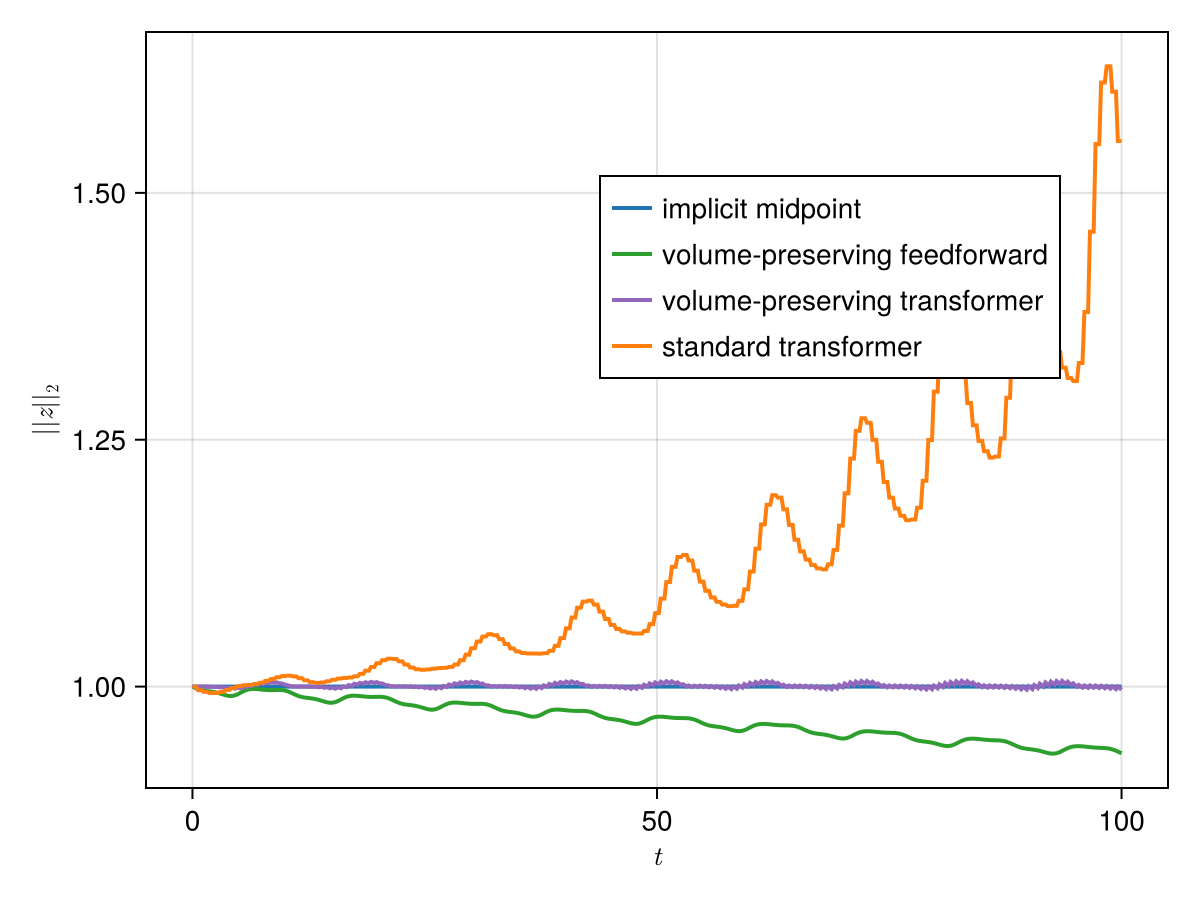
\includegraphics[width = .7\textwidth]{src/violate_invariant_long.png}
        \caption{\color{mred}Time evolution of invariant $I(z) = \sqrt{z_1^2 + z_2^2 + z_3^2} = ||z||_2$ for ``trajectory 1" up for the time interval $[0, 100]$. We see that for implicit midpoint this invariant is conserved and for the volume-preserving transformer it oscillates around the correct value.}
        \label{fig:VPFFvsVPT}
        \end{figure}
        }
    \item In Section 5.4, it is mentioned that the columns in the output of the VPT are linearly independent. This seems like a stretch, considering a zero vector-field could be considered. Perhaps this is rather a matter of invertibility? Is there a bound $T\leq{}d$? If so, this should be mentioned.
        {\color{mred} We rephrased the corresponding sentence to: ``The reason behind this could be that it is not sufficiently restrictive, i.e., the matrix which is made up of the three columns in the output of the transformer does not have full rank (i.e. is not invertible); a property that the volume-preserving transformer has by construction.''}
\end{enumerate}


\subsection*{Remarks}

\begin{enumerate}
    \item In terms of philosophy, why would long-range interactions/dependencies be interesting for first-order differential equations?
    \item Too much importance is given to reduced-order modelling in the introduction, considering no ROM is performed in the paper. Instead, more this space could be used to accurately introduce and describe the volume-preserving properties of the authors' architecture.
        
    
    {\color{mred} We reduced the discussion of reduced order modeling to the following: ``An application, where all of these developments intersect, is \textit{reduced-order modeling} , which can be split into an \textit{offline phase} and an \textit{online phase} (see \Cref{fig:OfflineOnlineSplit}).

        \begin{figure}[h]
        \centering
        \includestandalone[width=.5\textwidth]{src/tikz/offline_online}
        \caption{\color{mred}Visualization of offline-online split in reduced order modeling. The volume-preserving transformer presented in this work is \textit{used for the online phase}.}
        \label{fig:OfflineOnlineSplit}
        \end{figure}
        
        For the online phase we face the following challenges:
        
        \begin{itemize}
        \item[1. ] in many cases we need to recover the dynamics of our system from data alone (this is known as ``non-intrusive reduced order modeling"), 
        \item[2. ] if the big system exhibits specific structure (such as volume-preservation) it is often crucial to also respect this structure in the reduced model''.  
        \end{itemize}}

    \item As someone unfamiliar with volume-preserving multistep methods, I would have appreciated a comparison of the theoretical results: what is the impact of replacing the volume on the original space by the volume on the product space? Is that standard? Is one better than the other?
        {\color{mred} We added the following remark to highlight the similarities of our product structure with different work:
        
        \begin{rmrk*} 
            To our knowledge there is no literature on volume-preserving multi-step methods, there is however significant work on \textit{symplectic multi-step methods}. Of the two definitions of symplecticity for multi-step methods given in (Hairer et. al, 2006), that of \textit{\(G\)-symplecticity} is similar to the definition of volume preservation given here as it is also defined on a product space. The product structure through which we defined volume preservation also bears strong similarities to ``discrete multi-symplectic structures" defined in (Bridges and Reich, 2001) and (Y{\i}ld{\i}z et. al, 2024). 
        \end{rmrk*}

        }
    \item Assuming the ODE is unknown, how can one compute the first three time-steps? Would using the less-accurate VPFF for this prediction be accurate enough? If not, is the transformer faster and/or more accurate than the midpoint scheme?
        {\color{mred}
        We answer this in two parts:
        \begin{enumerate}
            \item 

            \item Regarding the comparison with implicit midpoint we added:

            ``In order to get an estimate for the different computational times we perform integration up to time 50000 for all four methods. On CPU we get:
            
            \begin{table}[h]
            \centering
            \begin{tabulary}{\linewidth}{R L L L L}
            \toprule
            \color{mred} Method & \color{mred} IM & \color{mred} VPFF & \color{mred} VPT & \color{mred} ST \\
            \toprule
            \color{mred} Training time & \color{mred} 2.51 seconds & \color{mred} 6.44 seconds & \color{mred} 0.71 seconds & \color{mred} 0.20 seconds \\
            \bottomrule
            \end{tabulary}
            
            \end{table}
            
            We see that the standard transformer is the fastest, followed by the volume-preserving transformer. The slowest is the volume-preserving feedforward neural network. We attempt to explain those findings:
            
            \begin{itemize}
            \item we assume that the standard transformer is faster than the volume-preserving transformer because the softmax can be quicker evaluated than our new activation function,
            \item we assume that implicit midpoint is slower than the two transformers because it involves a Newton solver and the neural networks all perform explicit operations,
            \item the very poor performance of the volume-preserving feedforward neural network is harder to explain. We suspect that our implementation performs all computations in serial and is therefore slower than the volume-preserving transformer by a factor of three, because we have \(\mathrm{L} = 3\) transformer units. It can furthermore be assumed to be slower by another factor of three because the feedforward neural network only predicts one time step at a time as opposed to three time steps at a time for the two transformer neural networks.
            \end{itemize}
            
            Another advantage of all neural network-based integrators over implicit midpoint is that it is easily suitable for parallel computation on GPU because all operations are explicit\footnotemark. The biggest motivation for using neural networks to learn dynamics comes however from non-intrusive reduced order modeling as discussed in the introduction; a traditional integrator like implicit midpoint is simply not suitable for this task as we need to recover dynamics from data.''
        \end{enumerate}

        
        }
    \item Some typos: ``those efforts was'' in the abstract, ``ob the Jacobian'' p. 3.
\end{enumerate}

\end{document}